%++++++++++++++++++++++++++++++++++++++++
% Don't modify this section unless you know what you're doing!
\documentclass[letterpaper,12pt]{article}
\usepackage{tabularx} % extra features for tabular environment
\usepackage{amsmath}  % improve math presentation
\usepackage{graphicx} % takes care of graphic including machinery
\usepackage[margin=1in,letterpaper]{geometry} % decreases margins
\usepackage[final]{hyperref} % adds hyper links inside the generated pdf file
\hypersetup{
	colorlinks=true,       % false: boxed links; true: colored links
	linkcolor=blue,        % color of internal links
	citecolor=blue,        % color of links to bibliography
	filecolor=magenta,     % color of file links
	urlcolor=blue         
}
%++++++++++++++++++++++++++++++++++++++++

\usepackage{titling}
\pretitle{\begin{flushright}}
\posttitle{\par\end{flushright}}
\preauthor{\begin{flushright}}
\postauthor{\par\end{flushright}}
\predate{\begin{flushright}}
\postdate{\par\end{flushright}}

\usepackage[font=small,skip=0pt]{caption}

% \usepackage[demo]{graphicx}
\usepackage{subcaption}
\usepackage{float}

\usepackage[style=ieee,backend=biber]{biblatex}
\addbibresource{report.bib}

\begin{document}

\title{\vspace{-2cm} Kavi Dey}
\author{\vspace{-0.4cm} E157 RF Design \\ Lab Partner: Zoe Worrall \\ Design Project 2}
\date{\vspace{-0.4cm} \today}
\maketitle

% modified from https://www.overleaf.com/latex/templates/sample-lab-report-for-u-of-r-phys-349/pgsyqngcyjxk
%++++++++++++++++++++++++++++++++++++++++

% abstract
% \begin{abstract}
% abstract here
% \end{abstract}

% sections
\section{Summary Information}
The secret message is "HMC". The maximum range that we predicted our receiver would work at was XX m.
The range where the signal reached the noise floor was XX m, and the range where the signal was no longer decodable on the oscilloscope was XX m.
\\
\\
\noindent
The analytical system temperature was XX K and the measured temperature was XX K. The analytical receiver IIP3 was XX dBm and the measured one was XX dBm.

\newpage
\section{Pictures of Received Data}
\begin{figure}[H]
	\begin{centering}
		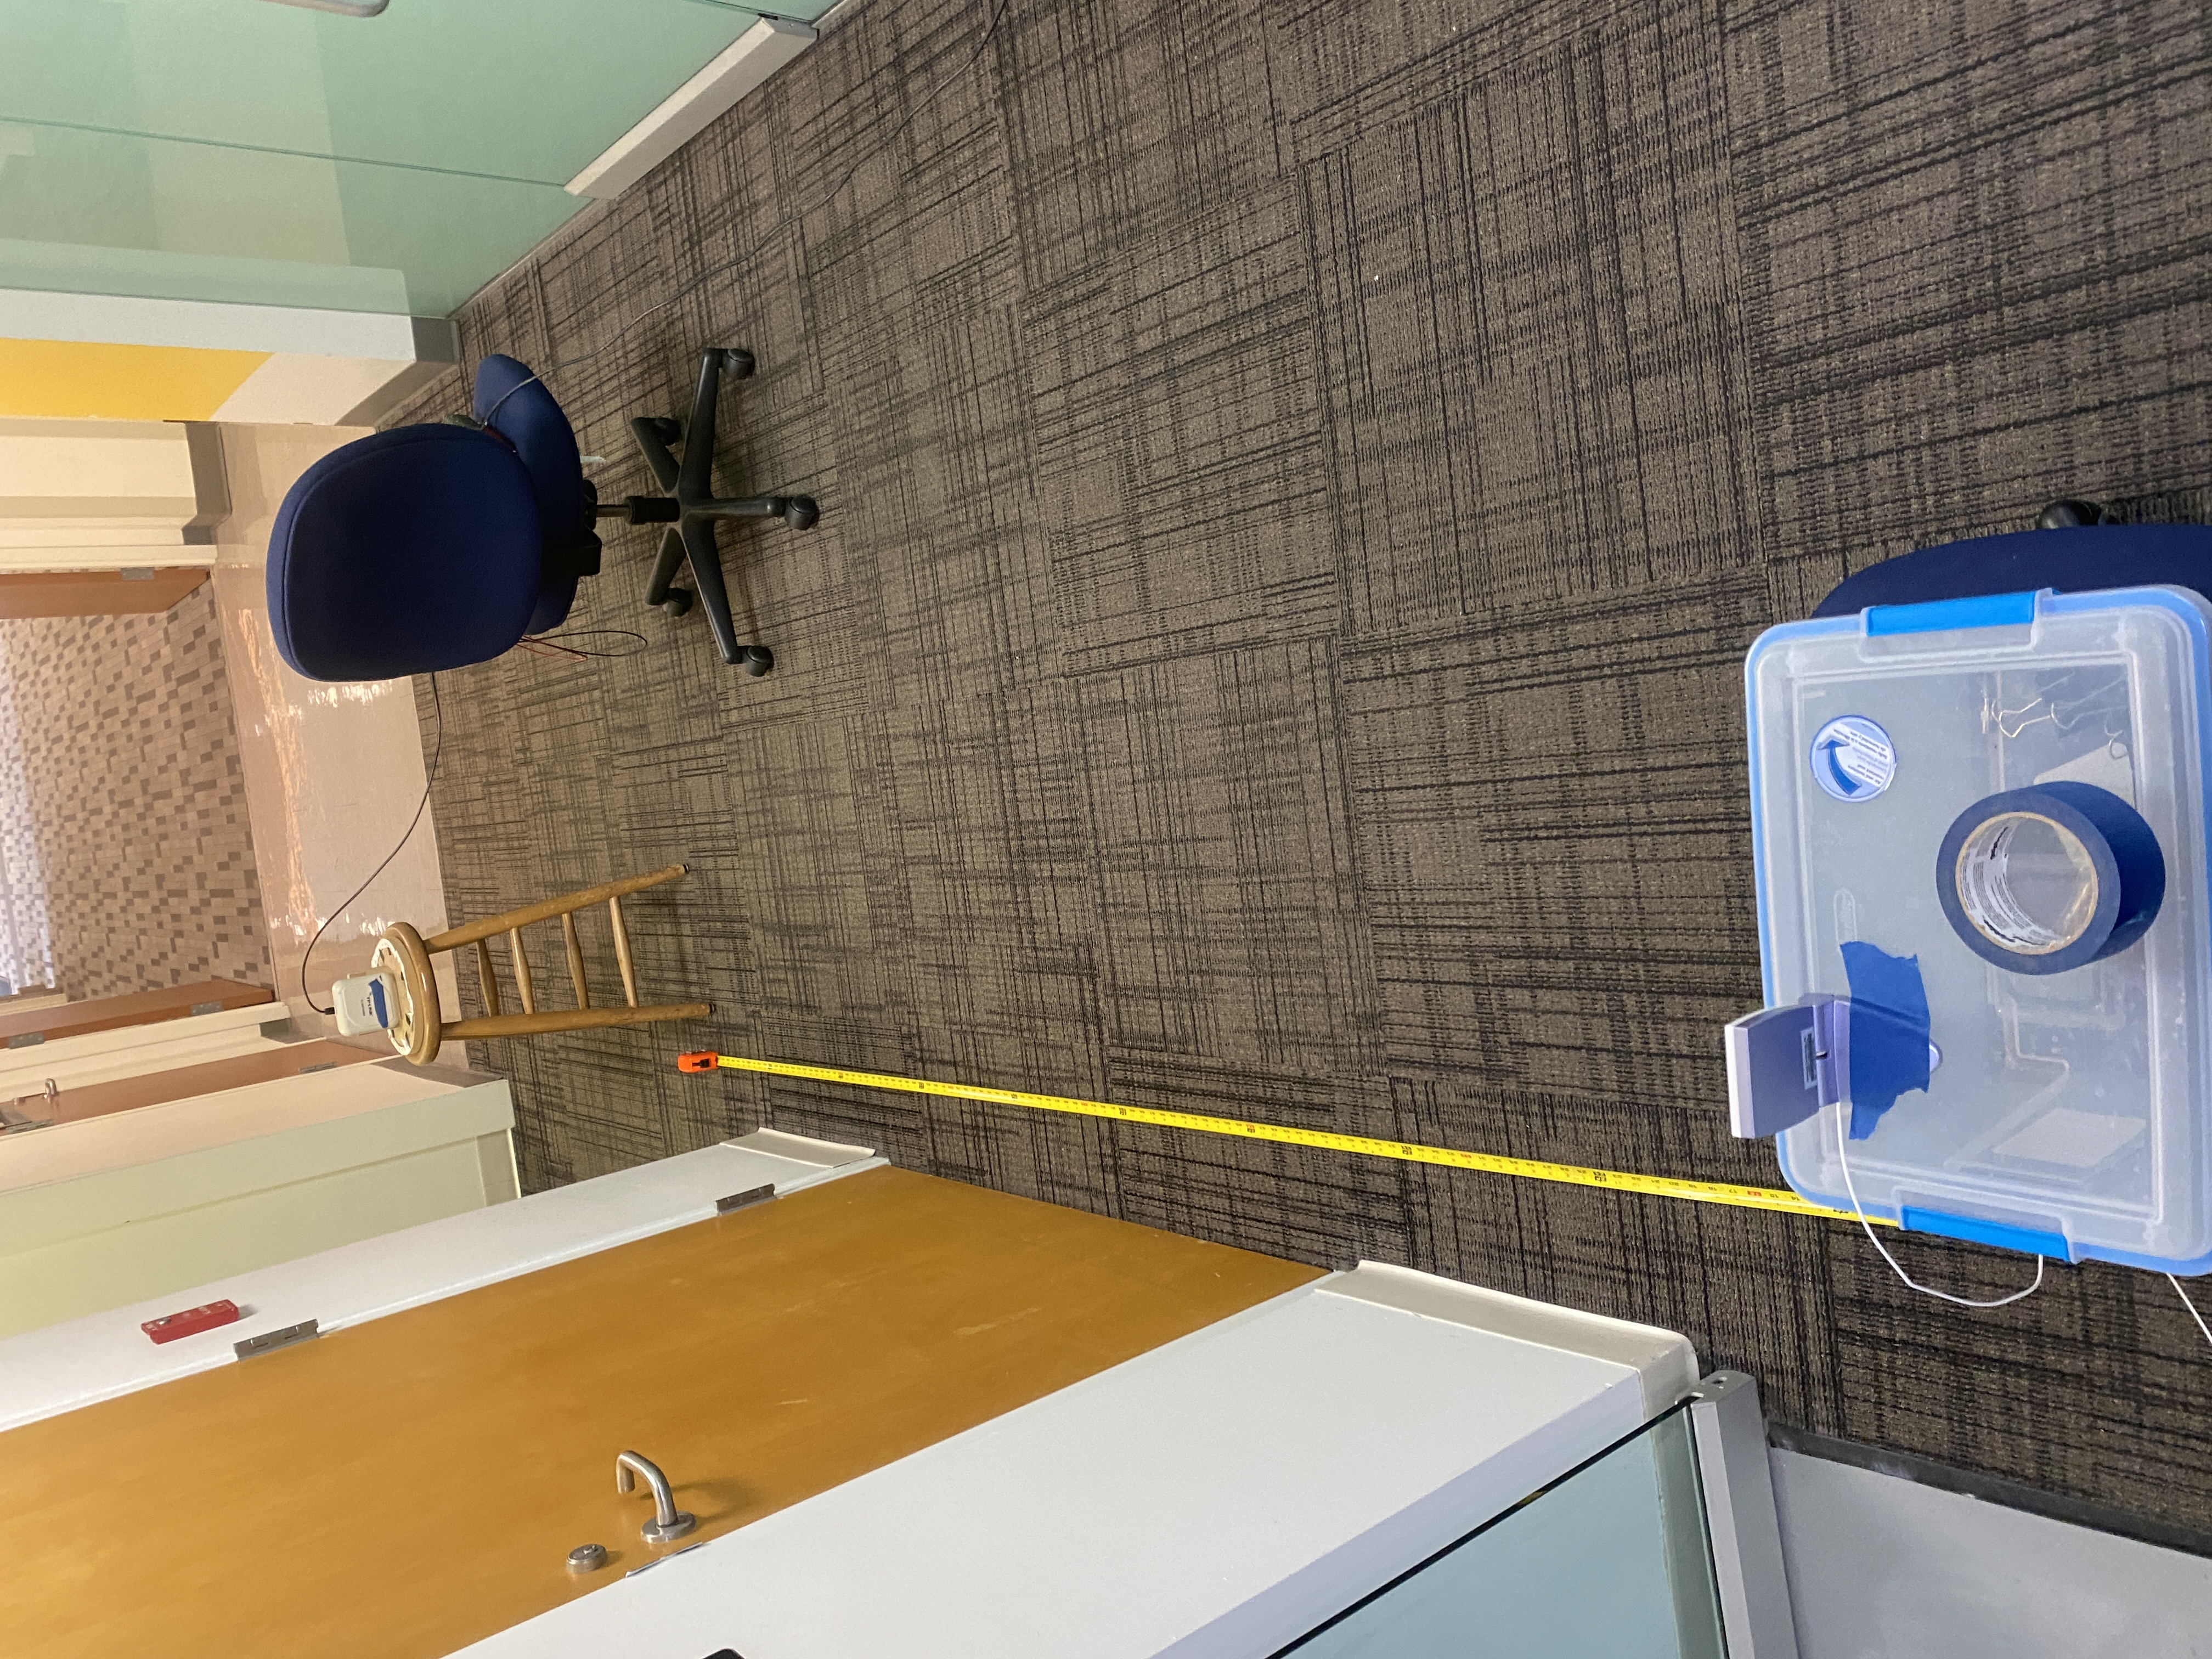
\includegraphics[width=0.5\columnwidth,angle=-90]{figures/3m.img}
		\caption{Picture of setup at 3 m range}
	\end{centering}
\end{figure}

\begin{figure}[H]
	\begin{centering}
		\includegraphics[width=0.5\columnwidth]{example-image-a}
		\caption{Oscilloscope trace at 3 m range}
	\end{centering}
\end{figure}

\begin{figure}[H]
	\begin{centering}
		\includegraphics[width=0.5\columnwidth]{example-image-a}
		\caption{Spectrum at 3 m range}
	\end{centering}
\end{figure}

\begin{figure}[H]
	\begin{centering}
		\includegraphics[width=0.5\columnwidth]{example-image-a}
		\caption{Picture of setup at max range}
	\end{centering}
\end{figure}

\begin{figure}[H]
	\begin{centering}
		\includegraphics[width=0.5\columnwidth]{example-image-a}
		\caption{Oscilloscope trace at max range}
	\end{centering}
\end{figure}

\begin{figure}[H]
	\begin{centering}
		\includegraphics[width=0.5\columnwidth]{example-image-a}
		\caption{Spectrum at max range}
	\end{centering}
\end{figure}


\newpage
\section{Oscilloscope Trace Decoding}
\begin{figure}[H]
	\begin{centering}
		\includegraphics[width=0.7\columnwidth]{example-image-a}
		\caption{Spectrum at max range}
	\end{centering}
\end{figure}

\newpage
\section{Antenna Information}
\begin{figure}[H]
	\begin{centering}
		\includegraphics[width=0.5\columnwidth]{example-image-a}
		\caption{XXXXX Antenna}
	\end{centering}
\end{figure}

\newpage
\section{Receiver Schematic}
\begin{figure}[H]
	\begin{centering}
		\includegraphics[width=0.5\columnwidth]{example-image-a}
		\caption{Picture of Receiver}
	\end{centering}
\end{figure}

\begin{figure}[H]
	\begin{centering}
		\includegraphics[width=0.5\columnwidth]{example-image-a}
		\caption{Receiver Schematic}
	\end{centering}
\end{figure}

\newpage
\section{Receiver Spectra}

\newpage
\section{Theoretical Signal and Noise Levels}

\newpage
\section{IP3 Distortion Characterization}

% \newpage
% \section{Discussions \label{sec:discussion}}
% Discussion of discrepancies between analytical, simulated and measured results.  Quantitatively justify differences between them, including any modifications you made to your models to make your simulations match your measurements better (e.g.: board parasitics).  Refer to prior figures in your report for supporting evidence in this discussion.

\section{Additional Notes}
All of the data, code, and figures are available in this github repo: \url{github.com/kavidey/e157/tree/main/dp_02}.
\begin{enumerate}
  \item \texttt{schematics/} has the pretty display schematics made in Altium
\end{enumerate}

% \newpage
% \section{Takeaways}
% One paragraph about one thing you learned about RF design doing this project.

% \newpage
% \section{Bibliography}
% \printbibliography

% referencing bibliography
% ~\cite{melissinos, Cyr, Wiki}

% figures
% \begin{figure}[ht] 
%     \centering \includegraphics[width=0.8\columnwidth]{sr_setup}
%     \caption{
%             \label{fig:samplesetup}
%             Every figure MUST have a caption.
%     }
% \end{figure}

% equations
% \begin{equation} \label{eq:aperp} % the label is used to reference the equation
%     u(\lambda,T)=\frac{8\pi hc\lambda^{-5}}{e^{hc/\lambda kT}-1},
% \end{equation}
%
% ~\ref{fig:samplesetup}

% tables
% \begin{table}[ht]
%     \begin{center}
%         \caption{Every table needs a caption.}
%         \label{tbl:bins} % spaces are big no-no withing labels
%         \begin{tabular}{|cc|}
%             \hline
%             \multicolumn{1}{|c}{$x$ (m)} & \multicolumn{1}{c|}{$V$ (V)} \\
%             \hline
%             0.0044151                    & 0.0030871                    \\
%             0.0021633                    & 0.0021343                    \\
%             0.0003600                    & 0.0018642                    \\
%             0.0023831                    & 0.0013287                    \\
%             \hline
%         \end{tabular}
%     \end{center}
% \end{table}
%
% Table~\ref{tbl:bins} is an example.

% \newpage

% bibliography
% \begin{thebibliography}{99}
%     \bibitem{levitator_paper}
%     Asier Marzo, Adrian Barnes, Bruce W. Drinkwater; TinyLev: A multi-emitter single-axis acoustic levitator. \textit{Rev. Sci. Instrum.} 1 August 2017; 88 (8): 085105. \href{https://doi.org/10.1063/1.4989995}{https://doi.org/10.1063/1.4989995}

%     \bibitem{levitator_instructions}
%     Instructables ultrasonic levitator materials and instructions. \href{https://www.instructables.com/Acoustic-Levitator/}{https://www.instructables.com/Acoustic-Levitator/}
% \end{thebibliography}
\end{document}